% Options here are passed to the article class.
% Most common options: 10pt, 11pt, 12pt
\documentclass[10pt]{datasheet}

% Input encoding and typographical rules for English language
\usepackage[utf8]{inputenc}
\usepackage[english]{babel}
\usepackage[english]{isodate}

% tikz is used to draw images in this example, but you can
% also use \includegraphics{}.
\usepackage{graphicx}

% These define global texts that are used in headers and titles.
\title{LC05: Stateless Find Nearest}
\author{Andrews54757}
\tags{logic-and-computation}
\date{December 2022}
\revision{Revision 1}
\begin{document}
\maketitle

\section{Features}

\begin{itemize}
\item{Stateless, uses quasi-based logic}
\item{Will not output more than one group at a time, even with random slice activation/deactivation timings}
\end{itemize}

\section{Applications}

\begin{itemize}
\item{Box groupers}
\end{itemize}

\section{General Description}
The LC05 find nearest dispenser outputs items from first filled dropper in line with each pulse. With an 8gt clock this will have an additional 8gt transition delay between groups. Items can be inserted during operation and the thing won't output multiple groups at same time by accident.
\vfill\break

\begin{figure}[h]
    \centering
    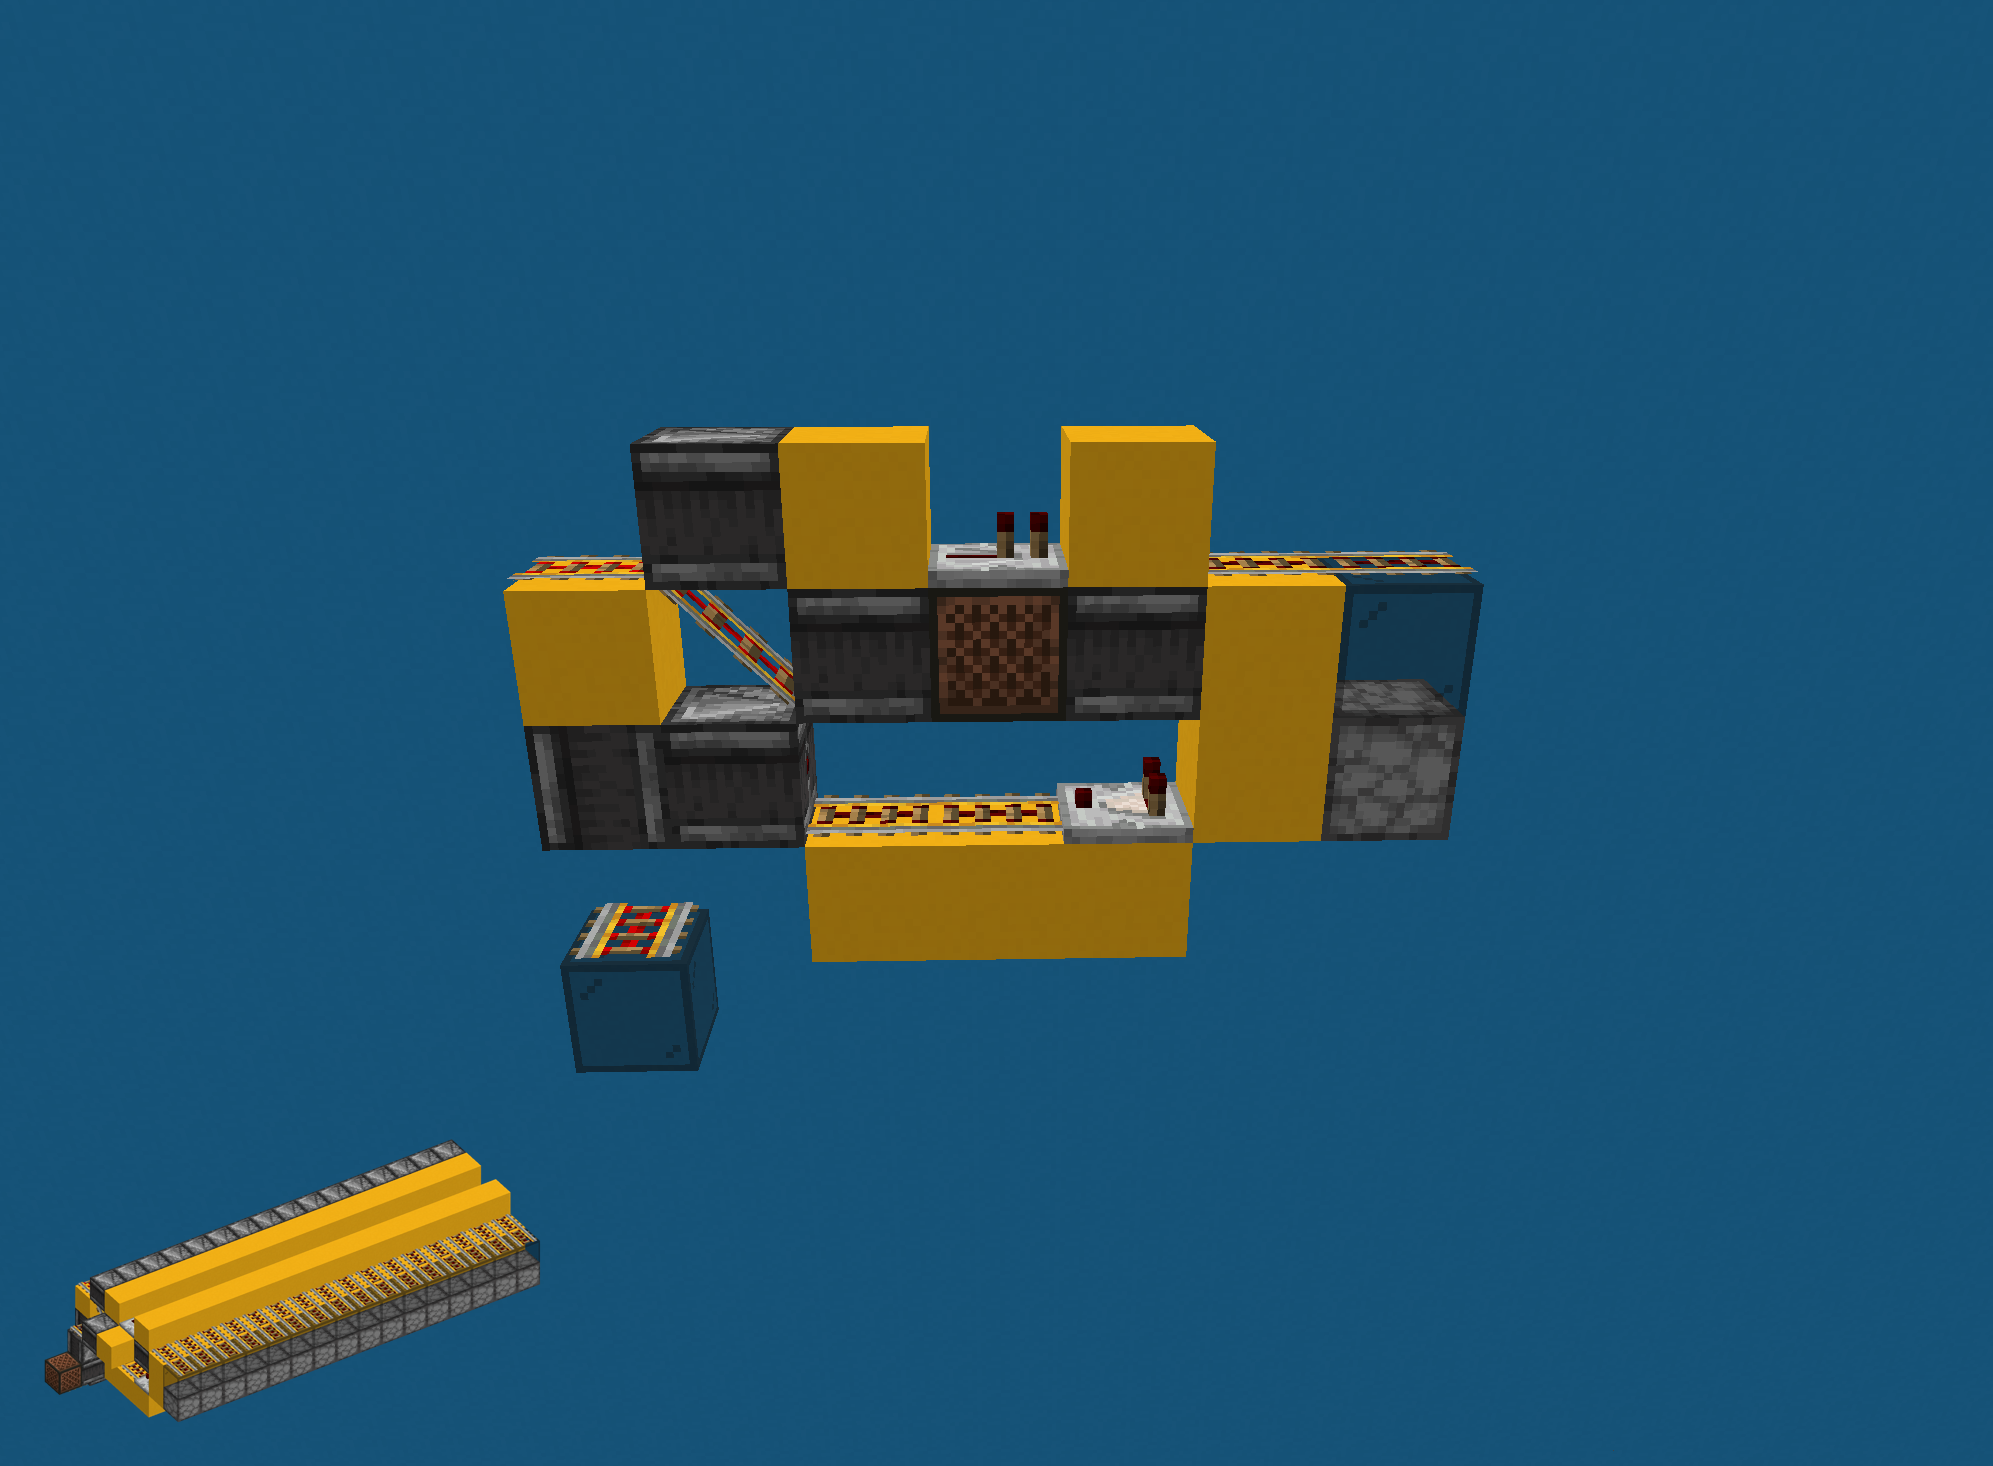
\includegraphics[width=0.48\textwidth]{dispense.png}
    \caption{\centering Stateless Group Dispenser}
\end{figure}

% For wide tables, a single column layout is better. It can be switched
% page-by-page.
\onecolumn

\section{Device Specifications}

\begin{table}[h]
    \caption{Inputs}
    \begin{tabularx}{\textwidth}{l | c | X}
        \thickhline
        \textbf{Name} & \textbf{Range} & \textbf{Description} \\
        \hline
        Clock signal & Pulse & Outputs an item with each pulse. \\
        \thickhline
\end{tabularx}
\end{table}

\begin{table}[h]
    \caption{Outputs}
    \begin{tabularx}{\textwidth}{l | c | X}
        \thickhline
        \textbf{Name} & \textbf{Range} & \textbf{Description} \\
        \hline
        Item Output & Item & Output item from first dropper in line. \\
        \thickhline
\end{tabularx}
\end{table}

\begin{table}[h]
    \caption{Device Specifications}
    \begin{tabularx}{\textwidth}{l | c c c | c | X}
        \thickhline
        \textbf{Parameter} & \textbf{Min.} & \textbf{Typ.} & \textbf{Max.} &
        \textbf{Unit} & \textbf{Conditions} \\
        \hline
        Throughput  & 8 & - & - & gt & Normal Usage \\
        \hline
        Latency    & 6 & - & - & gt & From input to dropper activation. \\
        \hline
        MC Version & 1.13 & 1.17.1 & - & MCV & Latest version at time of writing: 1.19.3\\
        \hline
        Dimensions & & 3 x 4 x 8 & & Blocks & \\
        \thickhline
\end{tabularx}
\end{table}
\newpage
\section{Testing Data}
\begin{table}[h]
\caption{Executed Tests}
\begin{tabularx}{\textwidth}{l | X}
    \thickhline
    \textbf{Test} & \textbf{Result} \\
    \hline
    Throughput test & Device was able to function with 8gt clocked input. \\
    \thickhline
\end{tabularx}
\end{table}

\section{Download Information}
\begin{table}[h]
    \caption{Download Information}
    \begin{tabularx}{\textwidth}{l | l | l | X}
        \thickhline
        \textbf{Identifier} & \textbf{MC} & \textbf{File} & \textbf{Description} \\
        \hline
        LC05 & 1.17.1 & \href{https://github.com/Soontech-Annals/Archive/blob/8413f90a054b6c415703bae02badeba7541344f6/Archive/logic-and-computation/LC05\%20Stateless\%20Find\%20Nearest/LC05\_stateless\_find\_nearest.litematic?raw=1}{LC05\_stateless\_find\_nearest.litematic} & Schematic of device. \\
        \hline
        \thickhline
    \end{tabularx}
\end{table}

\end{document}

